%% For double-blind review submission, w/o CCS and ACM Reference (max submission space)
\documentclass[sigplan,review,anonymous]{acmart}\settopmatter{printfolios=true,printccs=false,printacmref=false}
%% For double-blind review submission, w/ CCS and ACM Reference
%\documentclass[sigplan,review,anonymous]{acmart}\settopmatter{printfolios=true}
%% For single-blind review submission, w/o CCS and ACM Reference (max submission space)
%\documentclass[sigplan,review]{acmart}\settopmatter{printfolios=true,printccs=false,printacmref=false}
%% For single-blind review submission, w/ CCS and ACM Reference
%\documentclass[sigplan,review]{acmart}\settopmatter{printfolios=true}
%% For final camera-ready submission, w/ required CCS and ACM Reference
%\documentclass[sigplan]{acmart}\settopmatter{}


%% Conference information
%% Supplied to authors by publisher for camera-ready submission;
%% use defaults for review submission.
\acmConference[PL'18]{ACM SIGPLAN Conference on Programming Languages}{January 01--03, 2018}{New York, NY, USA}
\acmYear{2018}
\acmISBN{} % \acmISBN{978-x-xxxx-xxxx-x/YY/MM}
\acmDOI{} % \acmDOI{10.1145/nnnnnnn.nnnnnnn}
\startPage{1}

%% Copyright information
%% Supplied to authors (based on authors' rights management selection;
%% see authors.acm.org) by publisher for camera-ready submission;
%% use 'none' for review submission.
\setcopyright{none}
%\setcopyright{acmcopyright}
%\setcopyright{acmlicensed}
%\setcopyright{rightsretained}
%\copyrightyear{2018}           %% If different from \acmYear

%% Bibliography style
\bibliographystyle{ACM-Reference-Format}
%% Citation style
\citestyle{acmauthoryear}  %% For author/year citations
%\citestyle{acmnumeric}     %% For numeric citations
%\setcitestyle{nosort}      %% With 'acmnumeric', to disable automatic
                            %% sorting of references within a single citation;
                            %% e.g., \cite{Smith99,Carpenter05,Baker12}
                            %% rendered as [14,5,2] rather than [2,5,14].
%\setcitesyle{nocompress}   %% With 'acmnumeric', to disable automatic
                            %% compression of sequential references within a
                            %% single citation;
                            %% e.g., \cite{Baker12,Baker14,Baker16}
                            %% rendered as [2,3,4] rather than [2-4].


%%%%%%%%%%%%%%%%%%%%%%%%%%%%%%%%%%%%%%%%%%%%%%%%%%%%%%%%%%%%%%%%%%%%%%
%% Note: Authors migrating a paper from traditional SIGPLAN
%% proceedings format to PACMPL format must update the
%% '\documentclass' and topmatter commands above; see
%% 'acmart-pacmpl-template.tex'.
%%%%%%%%%%%%%%%%%%%%%%%%%%%%%%%%%%%%%%%%%%%%%%%%%%%%%%%%%%%%%%%%%%%%%%


%% Some recommended packages.
\usepackage{booktabs}   %% For formal tables:
                        %% http://ctan.org/pkg/booktabs
\usepackage{subcaption} %% For complex figures with subfigures/subcaptions
                        %% http://ctan.org/pkg/subcaption
                        \usepackage{amsmath}
\usepackage{amsthm}
\usepackage{amssymb}
\usepackage{hyperref}
%\usepackage{theorem}
%\usepackage{proof}
\usepackage{graphicx}
\usepackage{xspace}
%\usepackage{ebproof}
\usepackage{stmaryrd}
\usepackage{rotating,color,xcolor}
\usepackage{comment}
\usepackage{tikz}
\usepackage{thm-restate}


%macros
\newcommand{\set}[1]{\left\{#1 \right\}}
\newcommand{\tuple}[1]{\left(#1 \right)}
\newcommand{\atuple}[1]{\left\langle #1 \right\rangle}
\newcommand{\sem}[1]{ \llbracket #1 \rrbracket}
\newcommand{\dist}[1]{ \lVert #1 \rVert}
\newcommand{\mleft}{\leftarrowtriangle}
\newcommand{\mright}{\rightarrowtriangle}

\newcommand{\infix}[2]{(#1{:}#2)}
\newcommand{\pref}[1]{\infix{}{#1}}
\newcommand{\suf}[1]{\infix{#1}{}}

\newcommand{\ptime}{\textsc{PTime}\xspace}
\newcommand{\exptime}{\textsc{ExpTime}\xspace}
\newcommand{\texptime}{\textsc{2-ExpTime}\xspace}
\newcommand{\nlogspace}{\textsc{NLogSpace}\xspace}

\newcommand{\nat}{\mathbb N}


\newcommand{\A}{\mathcal A}
\newcommand{\R}{\mathcal R}
\newcommand{\F}{\mathcal F}
\newcommand{\Ss}{\mathcal S}
\newcommand{\Tt}{\mathcal T}
\newcommand{\Oo}{\mathcal O}
\newcommand{\M}{\mathcal M}
\newcommand{\Pp}{\mathcal P}
\newcommand{\final}{\mathit t}
\newcommand{\id}{Id}
\newcommand{\dom}{\mathrm{dom}}
\newcommand{\ran}{\mathrm{ran}}
\newcommand{\fin}{\mathit{t}}
\newcommand{\finite}{\mathit{ fin}}

\newcommand{\ie}{\textit{i.e.}~}

\newcommand{\mso}{\textsc{mso}\xspace}
\newcommand{\call}{\mathsf {call}}

%theorem
\newtheorem{theorem}{Theorem}
\newtheorem{lemma}[theorem]{Lemma}
\newtheorem{proposition}[theorem]{Proposition}
\newtheorem{claim}[theorem]{Claim}
\theoremstyle{definition}
\newtheorem{definition}[theorem]{Definition}
\newtheorem{example}[theorem]{Example}
\newtheorem{terminology}[theorem]{Terminology}
\theoremstyle{remark}
\newtheorem{remark}[theorem]{Remark}


\begin{document}

%% Title information
\title[Pebble Minimization of Polyregular Functions]{Pebble Minimization of Polyregular Functions}         %% [Short Title] is optional;
                                        %% when present, will be used in
                                        %% header instead of Full Title.
%\titlenote{with title note}             %% \titlenote is optional;
                                        %% can be repeated if necessary;
                                        %% contents suppressed with 'anonymous'
%\subtitle{Subtitle}                     %% \subtitle is optional
%\subtitlenote{with subtitle note}       %% \subtitlenote is optional;
                                        %% can be repeated if necessary;
                                        %% contents suppressed with 'anonymous'


%% Author information
%% Contents and number of authors suppressed with 'anonymous'.
%% Each author should be introduced by \author, followed by
%% \authornote (optional), \orcid (optional), \affiliation, and
%% \email.
%% An author may have multiple affiliations and/or emails; repeat the
%% appropriate command.
%% Many elements are not rendered, but should be provided for metadata
%% extraction tools.

%% Author with single affiliation.
\author{Nathan Lhote}
\authornote{with author1 note}          %% \authornote is optional;
                                        %% can be repeated if necessary
%\orcid{nnnn-nnnn-nnnn-nnnn}             %% \orcid is optional
\affiliation{
  %\position{Position1}
  %\department{Department1}              %% \department is recommended
  \institution{University of Warsaw}            %% \institution is required
  %\streetaddress{Street1 Address1}
  %\city{City1}
  %\state{State1}
  %\postcode{Post-Code1}
  \country{Poland}                    %% \country is recommended
}
\email{nlhote@mimuw.edu.pl}          %% \email is recommended



%% Abstract
%% Note: \begin{abstract}...\end{abstract} environment must come
%% before \maketitle command
\begin{abstract}
  We show that a polyregular word-to-word function is regular if and only its output size is at most linear in its input size. Moreover a polyregular function can be realized by: a transducer with two pebbles if and only if its output has quadratic size in its input, a transducer with three pebbles if and only if its output has cubic size in its input, \textit{etc}.

  Moreover the characterization is decidable and, given a polyregular function, one can compute a transducer realizing it with the \emph{minimal} number of pebbles.
  
  We apply the result to \mso interpretations from words to words. We show that \mso interpretations of dimension $k$ exactly coincide with $k$-pebble transductions.
\end{abstract}


%% 2012 ACM Computing Classification System (CSS) concepts
%% Generate at 'http://dl.acm.org/ccs/ccs.cfm'.
\begin{CCSXML}
<ccs2012>
<concept>
<concept_id>10011007.10011006.10011008</concept_id>
<concept_desc>Software and its engineering~General programming languages</concept_desc>
<concept_significance>500</concept_significance>
</concept>
<concept>
<concept_id>10003456.10003457.10003521.10003525</concept_id>
<concept_desc>Social and professional topics~History of programming languages</concept_desc>
<concept_significance>300</concept_significance>
</concept>
</ccs2012>
\end{CCSXML}

\ccsdesc[500]{Software and its engineering~General programming languages}
\ccsdesc[300]{Social and professional topics~History of programming languages}
%% End of generated code


%% Keywords
%% comma separated list
\keywords{pebble transducers, polyregular functions, minimization, MSO interpretations}  %% \keywords are mandatory in final camera-ready submission


\maketitle
%% Note: \maketitle command must come after title commands, author
%% commands, abstract environment, Computing Classification System
%% environment and commands, and keywords command.




\section*{Introduction}
\paragraph*{Regular and polyregular functions}
This article is about word-to-word functions, which we often call transductions.
Regular functions constitute an extensively studied class of functions which is characterized by many different computation models: two-way deterministic automata with outputs, streaming string transducers \cite{AlurC10}, \mso-transductions \cite{EngelfrietH01}, regular combinators \cite{AlurFR14} and regular list functions \cite{BojanczykDK18}.

In this article we consider \emph{pebble transducers} which were introduced in \cite{MiloSV03}. A pebble transducer is a deterministic finite state device which can mark a bounded number of positions of its input with pebbles. These pebbles follow a \emph{stack discipline}, which means that only the most recently placed pebble can be moved. This restriction ensures that the model only recognizes regular languages \cite{GlobermanH96}. On every transition the machine may append a finite word to the output.

In \cite{Bojanczyk18} the authors provides three equivalent characterizations of functions realized by pebble transducers, which are called \emph{polyregular functions}:
an imperative programming language with \textbf{for} loops, a functional programming language with limited access to recursion (\textit{e.g.}~\textbf{map} but not \textbf{fold}), compositions of simple basic functions using a Krohn-Rhodes-like decomposition.

Another characterization, in terms of \mso interpretations, is shown in \cite{BojanczykKL19}.

One difference between regular and polyregular functions is that regular functions have linear growth (\textit{i.e.}~the  the image of a word of length $n$ has length in $\Oo(n)$) while polyregular functions may have, as the name suggests, polynomial growth. In fact, as we will see, this is the only difference.

\paragraph*{Growth rate}
We study the growth of polyregular functions. One of our main motivations was the following question: can one decide if a polyregular function is regular?

The output size of a $k$-pebble transducer over an input of size $n$ is in $\Oo(n^k)$. This can be easily seen since the number of configurations (state and positions of pebbles) is in $\Oo(n^k)$. In particular, a regular function has linear growth since a two-way transducer is nothing more than a $1$-pebble transducer.

Our first main result is to show that the converse holds as well. This means in particular that a polyregular function is regular if and only if its growth is linear.

Our second result is a procedure to minimize the number of pebbles needed to realize a polyregular function.
In particular this gives a way to decide if a polyregular function is regular.


In \cite{BojanczykKL19}, the authors show that \mso interpretations capture exactly the polyregular functions. Their construction goes from an \mso interpretation of dimension $k$ to a pebble transducers with many more pebbles. However one can easily see that an \mso interpretation of dimension $k$ has growth in $\Oo(n^k)$. Applying our result we obtain that the blow-up in dimension is not necessary and an \mso-interpretation of dimension $k$ can always be computed by a $k$-pebble transducer. Since \mso interpretations of dimension $k$ can express $k$-pebble transductions we obtain our third result: \mso interpretations of dimension $k$ exaclty capture polyregular functions of growth $\Oo(n^k)$. This relies on the result from \cite{BojanczykKL19}, which says that \mso interpretations capture the polyregular functions.


\paragraph*{Outline}
In Section~\ref{sec:defs} we give the definition of polyregular function and pebble transducer. In Section~\ref{sec:results} we state our main results. In Section~\ref{sec:reg} we introduce the techniques used in this paper, and we show how to decide if a regular function is bounded.
In Section~\ref{sec:poly} we extend these techniques to show the main technical lemma of the article: one can decide if a transducer with $k+1$-pebbles can be turned into an equivalent  transducer with only $k$-pebbles.
In Section~\ref{sec:proofs}, using the lemma of Section~\ref{sec:poly}, we are able to prove the main theorems presented in Section~\ref{sec:results}.

\section{Polyregular functions}
\label{sec:defs}

Polyregular functions have been shown to be characterized by many different computational models \cite{Bojanczyk18,BojanczykKL19}. The model we will be using is that of pebble transducers which are automata that can place pebbles on a bounded number of positions following a stack discipline, meaning that only the most recently placed pebble can be moved.
We define in this section the model of pebble transducers and start with $1$-pebble transducers (usually called two-way transducers) which characterize the regular functions.

\paragraph{$1$-pebble transducers}
A $1$-pebble transducer, (usually known as a two-way transducer) of input alphabet $\Sigma$ and output alphabet $\Gamma$ is a two-way automaton (meaning that it has a reading head, called here a pebble, which can scan the word in both directions) which reads words over $\Sigma^*$, and has the ability to output words over $\Gamma^*$ on every transition. 
The output of a $1$-pebble transducer over some word is the concatenation of the outputs of its transitions along a run.
In Figure~\ref{fig:config} we represent a configuration of a $1$-pebble transducer:

\begin{figure}[h!]
  \centering

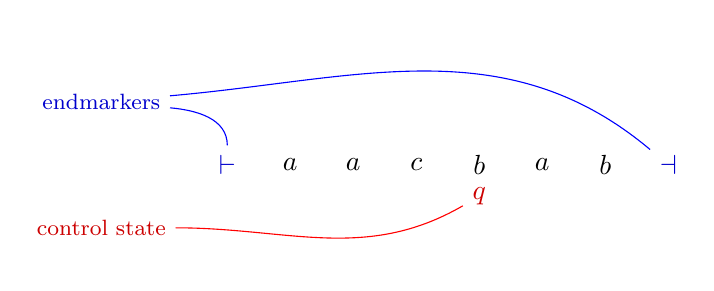
\begin{tikzpicture}[scale=.8]
\node[] (l) at (0,0) {{\color{blue!80!black}$\vdash$}};
\node[] () at (1,0) {$a$};
\node[] () at (2,0) {$a$};
\node[] () at (3,0) {$c$};
\node[] () at (4,0) {$b$};
\node[] () at (5,0) {$a$};
\node[] () at (6,0) {$b$};
\node[] (r) at (7,0) {{\color{blue!80!black}$\dashv$}};
\node[] (q) at (4,-.5) {{\color{red!80!black}$q$}};
\node[] (state) at (-2,-1) {\footnotesize{{\color{red!80!black}control state}}};
\draw[red] (state) edge[out=0,in=-150] (q) ;
\node[] (end) at (-2,1) {\footnotesize{{\color{blue!80!black}endmarkers}}};
\draw[blue] (end) edge[out=-5,in=90] (l) ;
\draw[blue] (end) edge[out=5,in=140] (r) ;

\end{tikzpicture}
\caption{Configuration of a $1$-pebble transducer.}
\label{fig:config}

\end{figure}

\begin{definition}[1-pebble transducer]\label{def:1pebble}
A $1$-pebble transducer is a tuple $(\Sigma,\Gamma, Q, q_I, q_F, \delta)$, which consists of:
\begin{itemize}
\item a finite input alphabet $\Sigma$ and a finite output alphabet $\Gamma$; 
\item a finite set of states $Q$;
\item two designated states $q_I$ and $q_F$: the initial and final one;
\item  a transition function of type  $$\delta : (\Sigma\cup\{\vdash,\dashv\}) \times Q \to Q\times\set{\mright,\mleft}\times\Gamma^*$$
The symbols  $\vdash$ and $\dashv$ are the endmarkers of the word. 
\end{itemize}
We assume that the transducer can only move to the right when it is on the left endmarker $\vdash$, and only to the left when  it is on the right endmarker $\dashv$. We also assume, without loss of generality, that the endmarkers don't output anything, meaning  $\delta(Q\times\set{\vdash,\dashv})\subseteq Q\times\set{\mright,\mleft}\times \set{\epsilon}$.
 \end{definition}
Let us define the behavior of the transducer over an input word $w\in\Sigma^*$.
The transducer actually reads the word ${\vdash} w{\dashv}$; and we denote by $\Sigma_{\vdash\dashv}$ the set  $\Sigma\cup\set{\vdash,\dashv}$.
\emph{A configuration} is seen as a word in the language ${\vdash}\Sigma^*{\dashv}$ with additional predicates in $Q$, such that only one position belongs to a predicate in $Q$. In Fig~\ref{fig:config2} we represent, using braces, the set of predicates that hold in a position, when there is more than one.

\begin{figure}[h!]

\begin{tikzpicture}
\node[] (l) at (0,0) {{\color{blue!80!black}$\vdash$}};
\node[] () at (1,0) {$a$};
\node[] () at (2,0) {$a$};
\node[] () at (3,0) {$c$};
\node[] () at (4,0) {$\{b{\color{red!80!black}q}\}$};
\node[] () at (5,0) {$a$};
\node[] () at (6,0) {$b$};
\node[] (r) at (7,0) {{\color{blue!80!black}$\dashv$}};
\end{tikzpicture}
\caption{Configuration of a $1$-pebble transducer.}
\label{fig:config2}
\end{figure}

The \emph{successor configuration} of a configuration $c$, when it exists, is obtained in the following way: apply $\delta$ to the pair $(a,q)$ corresponding to the letter $\{aq\}$, update the state and move the position of the pebble to the right or to the left accordingly.
The output of $c$ is the word in $\Gamma^*$ obtained by applying $\delta$.
\emph{A run} on $w$ is a sequence of configurations related by the successor relation defined above. The output of a run is the word obtained by concatenating the outputs of its configurations.

A configuration in $\{{\vdash}q_I\}\Sigma^*{\dashv}$ is called \emph{initial}, and a configuration in ${\vdash}\Sigma^*\{{\dashv}q_F\}$ is called \emph{final}. A run is \emph{accepting} if the first configuration is initial, the last one is final, and no other configuration is final. The accepting run over a word $w$, if it exists, is the unique (thanks to determinism) accepting run starting in $\{{\vdash}q_I\}w{\dashv}$.

A function is called \emph{regular} if it is realized by a $1$-pebble transducer.
\begin{example}
\label{ex:prefix}
Let us give an example of a transducer over alphabet $\set{a,b}$ which writes in unary in $\set{\lozenge}$ the length of the prefix of $a$'s of a word. We draw in Figure~\ref{fig:seq} the sequence of configurations of the run over the word $aaba$, whose image is $\lozenge\lozenge$.
\begin{comment}
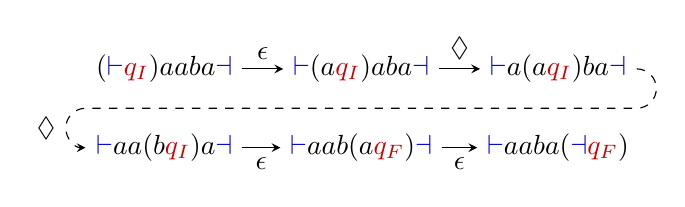
\begin{tikzpicture}[scale=1]
\node (1) at (0,0) {{$({\color{blue!80!black} \vdash}{\color{red!80!black}q_I})  aaba {\color{blue!80!black} \dashv}$}};

\node (2) at (2.5,0) {{$ {\color{blue!80!black} \vdash}  (a{\color{red!80!black}q_I})aba {\color{blue!80!black} \dashv}$}};

\node (3) at (5,0) {{$ {\color{blue!80!black} \vdash}  a(a{\color{red!80!black}q_I})ba {\color{blue!80!black} \dashv}$}};

\node (4) at (0,-1) {{$ {\color{blue!80!black} \vdash}  aa(b{\color{red!80!black}q_I})a {\color{blue!80!black} \dashv}$}};

\node (5) at (2.5,-1) {{${\color{blue!80!black} \vdash}  aab(a{\color{red!80!black}q_F}) {\color{blue!80!black} \dashv}$}};

\node (6) at (5,-1) {{${\color{blue!80!black} \vdash}  aaba ({\color{blue!80!black} \dashv}{\color{red!80!black}q_F})$}};


\draw[->,>=stealth] (1) edge[] node[above] {$\epsilon$} (2) ;
\draw[->,>=stealth] (2) edge[] node[above] {$\lozenge$} (3) ;
\draw[->,>=stealth,dashed] (6,0) arc(90:-90:.25)   -- (-1,-.5) arc(90:270:.25)  ;
\node at (-1.5,-.75) {$\lozenge$};
\draw[->,>=stealth] (4) edge[] node[below] {$\epsilon$} (5) ;
\draw[->,>=stealth] (5) edge[] node[below] {$\epsilon$} (6) ;
\end{tikzpicture}
\end{comment}

\begin{figure}[h!]

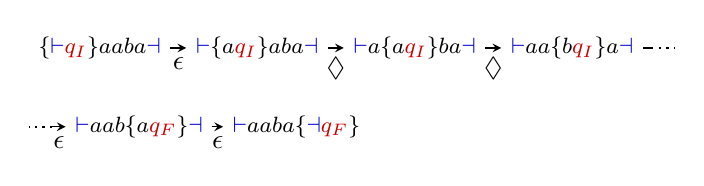
\begin{tikzpicture}[scale=1]
\node (1) at (0,0) {\footnotesize{$\{{\color{blue!80!black} \vdash}{\color{red!80!black}q_I}\}  aaba {\color{blue!80!black} \dashv}$}};


\node (2) at (2,0) {\footnotesize{$ {\color{blue!80!black} \vdash}  \{a{\color{red!80!black}q_I}\}aba {\color{blue!80!black} \dashv}$}};

\node (3) at (4,0) {\footnotesize{$ {\color{blue!80!black} \vdash}  a\{a{\color{red!80!black}q_I}\}ba {\color{blue!80!black} \dashv}$}};

\node (4) at (6,0) {\footnotesize{$ {\color{blue!80!black} \vdash}  aa\{b{\color{red!80!black}q_I}\}a {\color{blue!80!black} \dashv}$}};

\node (5') at (0.5,-1) {\footnotesize{${\color{blue!80!black} \vdash}  aab\{a{\color{red!80!black}q_F}\} {\color{blue!80!black} \dashv}$}};

\node (6') at (2.5,-1) {\footnotesize{${\color{blue!80!black} \vdash}  aaba \{{\color{blue!80!black} \dashv}{\color{red!80!black}q_F}\}$}};


\draw[->,>=stealth] (1) edge[] node[below] {$\epsilon$} (2) ;
\draw[->,>=stealth] (2) edge[] node[below] {$\lozenge$} (3) ;
\draw[->,>=stealth] (3) edge[] node[below] {$\lozenge$} (4) ;
\draw[-] (4) edge[] ++(1,0)  ;
\draw[dotted,thick] (7,0) edge ++(.3,0)   ;
\draw[->,>=stealth] (5') edge[] node[below] {$\epsilon$} (6') ;
\draw[<-,>=stealth] (5') edge[] node[below] {$\epsilon$} ++(-1.1,0)  ;
\draw[dotted,thick] (-.6,-1) edge  ++(-.3,0)   ;
\end{tikzpicture}

\caption{Sequence of configurations.}
\label{fig:seq}

\end{figure}

\end{example}



\paragraph{Pebble transducers}
In the literature (see \textit{e.g.}~\cite{Bojanczyk18}), a $k$-pebble transducer is a transducer with $k$ reading heads. The movement of these heads is subject to a stack discipline: only the pebble on top of the stack can move.
In this paper, we will work with a different yet equivalent definition of $k$-pebble transducers. Here a $k$-pebble transducer is a collection of $k$ distinct $1$-pebble transducers. The idea is that the transducer number $k$ can, along its run, call transducer $k-1$ to run over \emph{its} current configuration. Then transducer $k-1$ can itself call transducer $k-2$ to run over its current configuration, and so on. This is analogous of program composition: when a program $A$ calls a program $B$ as a subroutine, first program $B$ is executed on the current state of program $A$, then program $A$ resumes its computation.



\begin{definition}
  A $k$-pebble transducer of input alphabet $\Sigma$ and output alphabet $\Gamma$ is a tuple $\Tt=\atuple{T_1,\dots,T_{k}}$ such that for every $i\in\set{1,\ldots,n}$:
  \begin{itemize}
  \item  $T_i$ is a 1-pebble transducer, whose set of states is denoted $Q_i$;
  \item  The input alphabet of $T_i$ is $\Sigma$ with additional predicates in $Q_{>i}\quad$ ($Q_{>i}=\bigcup_{j>i}Q_j$);
  \item  The output alphabet of $T_i$ is $\Gamma \cup \set{\call_1,\ldots,\call_{i-1}}$.
  \end{itemize} 
  In particular, the input alphabet of $T_k$ is $\Sigma$ and the output alphabet of $T_1$ is $\Gamma$.
\end{definition}
The output letter $\call_j$ is to be interpreted as the transducer calling $T_j$ to run over its current configuration.
For every $i\in\set{1,\ldots, k}$,  the sequence $\atuple{T_1,\ldots,T_i}$ can be seen as an $i$-pebble transducer, of input alphabet $\Sigma_i=\Sigma\times \mathbf 2 ^{Q_{>i}}$ and output alphabet $\Gamma$. We denote this transducer by $\Tt_i$.

 \begin{definition}
We define, by induction on $k$, the function realized by a $k$-pebble transducer. The case $k=1$ has been treated in Definition~\ref{def:1pebble}. 

Consider a $k+1$ pebble transducer $\Tt=\atuple{T_1,\ldots,T_{k+1}}$, and let $Q_i$ be the set of states of $T_i$, for $i\leq k$.
By induction let $f_i:\Sigma_i^*\to \Gamma^*$ denote the transduction realized by $\Tt_i$, for $i\in \set{1,\ldots,k}$.
Let us define the image of a word $w$ of $\Sigma^*$ by the transduction realized by $\Tt$:
\begin{itemize}
  \item Let $r=c_1,\ldots,c_{n+1}$ be the accepting run of $T_{k+1}$ over $w$ and $\gamma_1,\ldots,\gamma_n$ be the outputs of the corresponding configurations.
  
  \item  For every $j\in\set{1,\ldots,n}$, let $u_j$ be the word obtained from $\gamma_j$ by replacing each occurrence of a letter $\call_i\in \set{\call_1,\ldots,\call_k}$ by $f_i(c_j')$ (where $c_j'$ is $c_j$ without endmarkers).
  
  \end{itemize}
  The image of $w$ by $\Tt$ is the word $u_1\cdots u_n$.

  A function is called \emph{polyregular} if it is realized by a pebble transducer.
\end{definition}

\begin{example}
Let us consider the $2$-pebble transducer $\Tt=\tuple{T_1,T_2}$, where $T_2$ realizes a function $f_{\mathrm{pref}}$ similar to the one defined in Example~\ref{ex:prefix}: it makes a number of calls to $T_1$ corresponding the length of the $a$ prefix of the input (separated by $\sharp$ symbols). $T_1$ realizes the transduction $f_{1}:(\set{a,b}\times \mathbf 2 ^{\set{q_I,q_F}})^*\mright \set{a,b}^*$ that copies a word, but erases the state predicates.
Then the transduction realized by $\Tt$ is the function $f:w\mapsto (w\sharp)^{|f_{\mathrm{pref}}(w)|}$.
The function $f$ copies an input word as many times as the length of the prefix of the word with only $a$'s.

The picture from Figure~\ref{fig:2peb} illustrates the behavior of $\Tt$: first $T_2$ runs over the input word, and each time $T_2$ produces a $\call_1$, this is interpreted as a call to $T_1$ to run over the current configuration. 

\begin{figure}[h!]

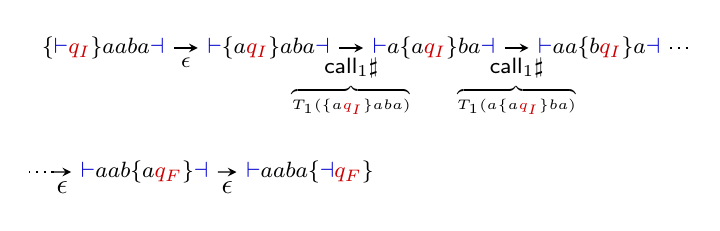
\begin{tikzpicture}[scale=1.05]
\node (1) at (0,0) {\footnotesize{$\{{\color{blue!80!black} \vdash}{\color{red!80!black}q_I}\}  aaba {\color{blue!80!black} \dashv}$}};


\node (2) at (2,0) {\footnotesize{$ {\color{blue!80!black} \vdash}  \{a{\color{red!80!black}q_I}\}aba {\color{blue!80!black} \dashv}$}};

\node (3) at (4,0) {\footnotesize{$ {\color{blue!80!black} \vdash}  a\{a{\color{red!80!black}q_I}\}ba {\color{blue!80!black} \dashv}$}};

\node (4) at (6,0) {\footnotesize{$ {\color{blue!80!black} \vdash}  aa\{b{\color{red!80!black}q_I}\}a {\color{blue!80!black} \dashv}$}};

\node (5') at (0.5,-1.5) {\footnotesize{${\color{blue!80!black} \vdash}  aab\{a{\color{red!80!black}q_F}\} {\color{blue!80!black} \dashv}$}};

\node (6') at (2.5,-1.5) {\footnotesize{${\color{blue!80!black} \vdash}  aaba \{{\color{blue!80!black} \dashv}{\color{red!80!black}q_F}\}$}};

\draw[->,>=stealth] (1) edge[] node[below] {\footnotesize{$\epsilon$}} (2) ;
\draw[->,>=stealth] (2) edge[] node[below] {\footnotesize{$\call_1 \sharp$}} (3) ;
\draw[->,>=stealth] (3) edge[] node[below] {\footnotesize{$\call_1 \sharp$}} (4) ;
\draw[dotted,thick] (4) edge[] ++(1.1,0) ;
\draw[->,>=stealth] (5') edge[] node[below] {$\epsilon$} (6') ;
\draw[<-,>=stealth] (5') edge[] node[below] {$\epsilon$} ++(-1.1,0)  ;
\draw[dotted,thick] (-.6,-1.5) edge  ++(-.3,0)   ;

\node (2) at (3,-.6) {\tiny{$\overbrace{T_1(  \{a{\color{red!80!black}q_I}\}aba)}$}};

\node (2) at (5,-.6) {\tiny{$\overbrace{T_1( a\{a{\color{red!80!black}q_I}\}ba)}$}};


\end{tikzpicture}
\caption{Run of a $2$-pebble transducer.}
\label{fig:2peb}
\end{figure}

By definition $f_1(  \{a{\color{red!80!black}q_I}\}aba)=f_1(  a\{a{\color{red!80!black}q_I}\}ba)=aaba$, hence we obtain $f(aaba)= aaba\sharp aaba\sharp$.
\end{example}
  

\begin{terminology}
  Let $f:\Sigma^*\to \Gamma^*$ be a word to word function.
  We say that $f$ has \emph{degree $k$ growth} (or, abusing notations, that it is \emph{in $\Oo(n^k)$}) if the size of the image of a word of size $n$ is in $\Oo(n^k)$.
  For degrees $0$, $1$ we shall use respectively the terms \emph{bounded} and \emph{linear growth}.
  %Moreover $f$ is \emph{strictly linear} if it is linear and not bounded.
  
\end{terminology}
The number of pebbles bounds in an obvious way the degree of a polyregular function:
\begin{proposition}
  \label{prop:degree}
The function realized by a transducer with $k$ pebbles is in $\Oo(n^k)$.
\end{proposition}


\begin{proof}
This is easily shown by observing that the number of configurations of a $k$-pebble transducer over a word of size $n$ is in $\Oo(n^k)$.
\end{proof}


\section{Results}
\label{sec:results}
We start by stating our results. First, the growth degree characterizes the number of necessary pebbles:
\begin{restatable}[Characterization]{theorem}{onkthm}
    \label{thm:onk}
    A polyregular function is in $\Oo(n^k)$ if and only if it can be realized by a transducer with $k$ pebbles.
\end{restatable}
Moreover, the characterization above is decidable and one can actually minimize the number of pebbles:
\begin{restatable}[Minimization]{theorem}{minthm}
    \label{thm:min}
    Given a polyregular function $f$ one can compute an equivalent pebble transducer with the minimal number of pebbles. In particular, one can decide if a polyregular function is regular.
\end{restatable}
Finally as a consequence (using the result from \cite[Theorem~7]{BojanczykKL19}) we obtain a correspondence between the dimension of \mso interpretations and the number of pebbles of pebble transducers.
\begin{restatable}[\mso-dimension]{theorem}{msothm}
    \label{thm:mso}
    A word-to-word function can be defined by an \mso interpretation of dimension $k$ if and only if it can be realized by a $k$-pebble transducer.
\end{restatable}
We now spend the rest of the article showing the above results. We start by introducing our main tool, the notion of transition morphism of a $1$-pebble transducer. We first characterize the regular functions, then we tackle the general case of degree $k$ growth in the final section.

We show in Section~\ref{sec:reg} how to decide if a regular function is bounded.  In Section~\ref{sec:poly} we prove the main lemma of the article, Lemma~\ref{lem:name}, which tells, given a $k$-pebble transducer, if one can construct an equivalent $k-1$-pebble transducer. Then, using Lemma~\ref{lem:name}, we prove the theorems above as corollaries.
%But first we need to define the notion of transition monoid of a $1$-pebble transducer.


\section{Deciding if a regular function is bounded}
\label{sec:reg}
We start by showing how to decide if a regular function is bounded or not. This not very deep result will serve as a stepping stone (as well as a warm-up) for the main contribution of the article.
To characterize bounded regular function, our main tool will be the usual notion of transition morphism of a 1-pebble transducer.

\begin{comment}
    A regular function has at most linear growth, but its output may be smaller than that. Let us show that there is a dichotomy: either a regular function has linear or bounded output size. This is not very hard to see: intuitively, either there is an input word with a part that can be pumped and which produces something, and then the length of the output is linear in the number of times the loop is pumped; or there is no such part, which means that any pumpable part can be removed without changing the output length, hence the output size is bounded.
    This not very deep result will serve as a stepping stone for the main contribution of the article.
\end{comment}

\subsection{Transition morphism of 1-pebble transducers}
We present here the tool used to summarize the behavior of a $1$-pebble transducer, called its transition monoid (resp. morphism). We map each word $w$ to an element of the monoid which gives the following kind of information \textit{e.g.}: if the automaton enters the word from the left in state $q$, then it exits to the left in state $q'$, \textit{etc}.
Moreover, we will sometimes need to record information about the output produced in such a pass of the transducer; this information can be for instance the whole output (in which case the monoid is infinite) or information of the kind ``a letter $a$ has been produced at least once'' (here we recover finiteness).

  
   
\begin{definition}[Transition monoid/morphism]%[Transition monoid of a 1-pebble transducer]
Let $T$ be a 1-pebble transducer with set of states $Q$ and output alphabet $\Gamma$.
%Let $N$ be a monoid, and let $\star$ be its multiplication.

We define the (infinite) transition monoid $M$ of $T$ as follows:
\begin{itemize}
\item its elements are functions of the form

$f:Q\times\set{\mright,\mleft}\to Q\times\set{\mright,\mleft}\times \Gamma^*$;
\item the composition $\cdot$ is defined as follows. Let $f, g$ be two elements of $M$, $q\in Q$ and $d\in\set{\mright, \mleft}$. We define the \emph{transition sequence} between 
$f$ and $g$ starting from $(q,d)$ and its \emph{output sequence} to be respectively the sequences $(q_i,d_i)_{i\in[0,n]}$ and  $(w_i)_{i\in[1,n]}$ satisfying the following conditions: 
\begin{itemize}
\item $(q_0,d_0)=(q,d)$;
\item two cases:
\begin{itemize}
  \item either $n=1$ and $d_1\neq d_0$
  \item or, $d_0=d_1$, $d_{n-1}=d_{n}$ and $d_i\neq d_{i+1}$ for every $i\in[1,n-2]$;
\end{itemize}  
\item if $d_0=\mright$

then for every even $i$,
$f(q_i,d_i)=(q_{i+1},d_{i+1}, w_{i+1})$ and for every odd $i$, $g(q_i,d_i)=(q_{i+1},d_{i+1}, w_{i+1})$;
\item if $d_0=\mleft$

then for every even $i$,
$g(q_i,d_i)=(q_{i+1},d_{i+1}, w_{i+1})$ and for every odd $i$, $f(q_i,d_i)=(q_{i+1},d_{i+1}, w_{i+1})$. 
\end{itemize}
We set $(f\cdot g) (q,d)$ to be $(q_n, d_n, w_1\cdot \dots\cdot w_n)$.
\end{itemize}
We give in Fig~\ref{fig:tran-seq} an illustration the transition sequence of $f,g$ starting in $(q,\mright)$.
\begin{figure}[h!]
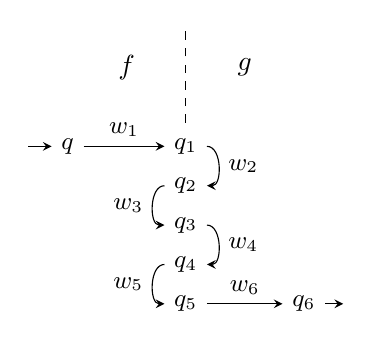
\begin{tikzpicture}
\node[] (0) at (0,0) {\small{$q$}};
\node[] (1) at (1.5,0) {\small{$q_1$}};
\node[] (2) at (1.5,-.5) {\small{$q_2$}};
\node[] (3) at (1.5,-1) {\small{$q_3$}};
\node[] (4) at (1.5,-1.5) {\small{$q_4$}};
\node[] (5) at (1.5,-2) {\small{$q_5$}};
\node[] (6) at (3,-2) {\small{$q_6$}};

\draw[<-,>=stealth] (0) -- node[above] {} (-.5,0);
\draw[->,>=stealth] (0) -- node[above] {\small{$w_1$}} (1);
\draw[->,>=stealth] (1) to[out=0,in=0] node[right] {\small{$w_2$}} (2);
\draw[->,>=stealth] (2) to[out=180,in=180] node[left] {\small{$w_3$}} (3);
\draw[->,>=stealth] (3) to[out=0,in=0] node[right] {\small{$w_4$}} (4);
\draw[->,>=stealth] (4) to[out=180,in=180] node[left] {\small{$w_5$}} (5);
\draw[->,>=stealth] (5) -- node[above] {\small{$w_6$}} (6);
\draw[->,>=stealth] (6) -- node[above] {} (3.5,-2);

\draw[dashed] (1.5,.3) -- (1.5,1.5);
\node[] at (.75,1) {$f$};
\node[] at (2.25,1) {$g$};

\end{tikzpicture}

\caption{Transition sequence of $f,g$ starting in $(q,\mright)$.}
\label{fig:tran-seq}
\end{figure}


\begin{comment}
We will mainly instantiate $M_N$ in the following three cases: 
\begin{enumerate}
\item $N$ is the monoid $\Gamma^*$ of words over $\Gamma$.
\item $N$ is the two element monoid $\mathbf 2$ with operation $\max$.
\item $N$ is the singleton monoid $\mathbf 1$.
\end{enumerate}
In the last case, the third component of the codomain of the elements of $M_{\mathbf 1}$ is useless, one can be see them as functions of type $Q\times\set{\mright,\mleft}\to Q\times\set{\mright,\mleft}$.
\end{comment}


We now define the transition morphism associated with transducer $T$.
Let $\mu:(\Sigma_{\vdash\dashv})^*\to M$ be defined as follows:
$$\text{For every } d\in \set{\mright,\mleft}\qquad\mu(a)(q,d)=\delta(a,q)$$

\begin{comment}
Let $\Delta\subseteq \Gamma$. We define the morphism $\mu_\Delta:(\Sigma_{\vdash\dashv})^*\to M_{\mathbf 2}$ as follows. Let $\chi_\Delta:\Gamma^*\to \mathbf{2}$ be the morphism defined on letters as follows $\chi_\Delta(\gamma)=1$ if $\gamma\in \Delta$ and $\chi_\Delta(\gamma)=0$ otherwise. We set for every $d\in\set{\mright,\mleft}$: 

$$\text{If } \delta(a,q)=(q',d',w) \text{ then } \mu_\Delta(a)(q,d)=(q',d',1_\Delta(w))$$


We define the morphism $\mu_{\mathbf{1}}:(\Sigma_{\vdash\dashv})^*\to M_{\mathbf 1}$ as follows. For every $d\in\set{\mright,\mleft}$,
$$\text{if } \delta(a,q)=(q',d',w) \text{ then }  \mu(a)(q,d)=(q',d') $$

\end{comment}


Finally, let $a\in  \Gamma$, we consider the morphism $\chi_a:\Gamma^*\rightarrow \set{0,1}$ defined by $\chi_a(a)=1$, and $\chi_a(b)=0$ if $b\neq a$, which says if a word contains at least one letter $a$.
We can naturally extend this to a morphism $\chi_a:M\rightarrow M_{\set{0,1}}$, with $M_{\set{0,1}}= Q\times\set{\mright,\mleft}\to Q\times\set{\mright,\mleft}\times \set{0,1}$.
In explicit terms, for $f\in M$, if $f(p,d)=(q,e,w)$ we have $\chi_a(f)(p,d)= (q,e,\chi_a(w))$.
We denote by $\mu_a$ the composition $\chi_a\circ \mu$.
\end{definition} 

\begin{example}
  \label{ex:transition}
    Let us consider the transducer given in Example~\ref{ex:prefix}.
    Its transition function is:

    $\delta: \begin{array}{crclrcl}
        &(\vdash,q_I) &\mapsto& (q_I,\mright,\epsilon) \\
        &(a,q_I)& \mapsto& (q_I,\mright,\lozenge) & (a,q_F)& \mapsto& (q_F,\mright,\epsilon)\\
        &(b,q_I)& \mapsto& (q_F,\mright,\epsilon) & (b,q_F)& \mapsto & (q_F,\mright,\epsilon)\\
        &(\dashv,q_I)& \mapsto& (q_F,\mright,\epsilon) & (\dashv,q_F)& \mapsto & (q_F,\mright,\epsilon)\\
    \end{array}$

\noindent As an example let us consider $f=\mu_{\lozenge}(ab)=\mu_{\lozenge}(aaababa)$, then $f: (q_I,\mright)$ $\mapsto (q_F,\mright,1)$. This means that the word $ab$ (as well as the word $aaababa$) goes from $q_I$ to $q_F$ from left to right, producing at least one symbol ${\lozenge}$.
\end{example}


\subsection{Producing triples and bounded regular functions}
Now that we have defined the transition morphism of a 1-pebble transducer, we can introduce the notion of \emph{producing triple} which characterizes non-boundedness. Intuitively, a producing triple means a loop in the run of the transducer that produces a non-empty output and can thus be pumped to produce arbitrarily large outputs.


\begin{definition}[Producing triple]
Let $T=(\Sigma,\Gamma,Q,q_I,q_F, \delta)$ be a 1-pebble transducer, and let $a\in \Gamma$. Let $(x, e, y)\in \mu_a( { \vdash}\Sigma^*)\times \mu_a( \Sigma^*)\times \mu_a( \Sigma^*{ \dashv})$.

We say that the triple $(x,e,y)$ is \emph{$a$-producing} if the transition sequence of $(xe,ey)$ starting from $(q_I,\mright)$, 
$(q_i,d_i)_{i\in[0,n]}$ satisfies the following conditions:
\begin{itemize}
\item $(q_n,d_n)=(q_F,\mright)$;
\item $e$ is idempotent i.e. $e\cdot e=e$;
\item there exists $i\in [1,n-1]$ such that $e(q_i,d_i)$ is of the form $(q,d,1)$.
\end{itemize}
\end{definition}
\begin{example}
  Using the same transducer as in Example~\ref{ex:transition}, we have that $(\mu_\lozenge({\vdash} aa),\mu_\lozenge(aba),\mu_\lozenge(ba{\dashv}))$, for instance, is a $\lozenge$-producing triple.

\end{example}


\begin{definition}
Let $f:\Sigma^*\to \Gamma^*$ be a function and $a\in\Gamma$. We say that $f$ is \emph{bounded} (resp.~\emph{linear}, \textit{etc}) \emph{in $a$} if $\pi_a\circ f: \Sigma^*\to a^*$ is bounded (resp. linear, \textit{etc}), where $\pi_a:\Gamma^*\to a^*$ is the morphism erasing non $a$ letters:
\begin{align*}
\pi_a(b)&=a \text{ if }  b=a \\
&= \epsilon \text{ otherwise.}
\end{align*}
 \end{definition}
The following lemma states that having a producing triple characterizes the functions that are unbounded.
\begin{lemma}\label{thm:linear}
A $1$-pebble transducer is bounded in $a$ if and only if it has no $a$-producing triple.
\end{lemma}
For the proof of the lemma, we will use a notion of factorization in a morphism, which will also be used in Section~\ref{sec:poly}.

\begin{definition}
    Let $\mu:\Sigma^*\to M$ be a monoid morphism and let $w$ be in $ \Sigma^*$.
    A $k$-factorization of $w$ in the morphism $\mu$ is given as a tuple of words $(w_0,x_{1},y_1,z_1,w_1,\ldots,x_k,y_k,z_k, w_k)$ verifying:
    \begin{itemize}   
        \item  $w=w_0x_1y_1z_1w_1\cdots x_ky_kz_kw_k$
        \item for all $i\in [1,k]$, $\mu(x_i)=\mu(y_i)=\mu(z_i)=\mu(x_ix_i)$
    \end{itemize}
    We say that such a factorization is \emph{according to} the tuple $(m_0,e_1,m_1,\ldots,e_k,m_k)$ if for all $i\in [0,k]$, $\mu(w_i)=m_i$ and for all $i\in [1,k]$, $\mu(x_{i})=e_i$.
\end {definition}

\begin{proof}[Proof of Lemma~\ref{thm:linear}]
    We know that a $1$-pebble transducer realizes a linear function, from Proposition~\ref{prop:degree}.
    Let $T$ be a $1$-pebble transducer realizing a function $f:\Sigma^*\to \Gamma^*$, and let $a\in \Gamma$.

    Let us first assume that there exists an $a$-producing triple $(m_0,e_1,m_1)$, and let $w$ be a word such that ${\vdash} w{\dashv }$ has a $1$-factorization $(w_0,x_1,y_1,z_1,w_1)$ according to this triple.
    Then we show that since $(m_0,e_1,m_1)$ is $a$-producing, $|f(w_0x_1y_1^nz_1w_1)|=\Theta(n)$.
    By definition of $a$-producing triple, the output while reading a $y_1$ factor is non-empty, hence $f$ is not bounded.

    Let us now assume that there are no $a$-producing triples.
    By a Ramseyan argument, there exists an integer $d$ such that any word of length greater than $d$ has a $1$-factorization.
    Let $w$ be a word with a $1$-factorization $(w_0,x_1,y_1,z_1,w_1)$. Since there are no $a$-producing triple, $(\mu_a(w_0),\mu_a(y_1),\mu_a(w_1))$ is not $a$-producing. This means that the outputs corresponding to the factor $y_1$ in the run over $w$ are all empty, and thus we have $|f(w_0x_1y_1z_1w_1)|=|f(w_0x_1z_1w_1)|$.
    Hence we have $\set{|f(w)|\mid\ w\in \Sigma^*}=\set{|f(w)|\mid\ w\in \Sigma^{\leq d}}$, hence $f$ is bounded.
\end{proof}



\section{Deciding if a polyregular function is in $\Oo(n^k)$}
\label{sec:poly}

Now that we have solved the case of 1-pebble transducers, we move on to general case: deciding if a $k+1$-pebble transduction can be realized by a $k$-pebble transducer. The main idea is, given $\atuple{T_1,\ldots,T_{k+1}}$, to modify $T_{k+1}$ so that it calls $T_k$ only when ``necessary''. Then, if this modified $T_{k+1}$ is bounded in $\set{\call_k}$, it means that the function can actually be realized by a transducer with $k$ pebbles.

In order to obtain Lemma~\ref{lem:name}, the main lemma of the section (actually of the article), we need several tools which we present below.

One first useful tool we will be using is that of \mso-labelling of words, \textit{i.e.}~labelling each letter with some regular information.
More formally an \mso-labelling is a function of type $\ell:\Sigma^*\rightarrow (\Sigma\times L)^*$, which does not change the $\Sigma$ component. It is given some unary \mso-formulas $\phi_1(x),\cdots,\phi_p(x)$ and a function $g:\mathbf 2^{\set{1,\ldots, p}}\rightarrow L$. Given a word $u\in \Sigma^*$ we define $v=\ell(u)$ by $v[i]=(u[i],l)$, with $l=g(I)$ such that $u\models \bigwedge_{j\in I}\phi_j(i)\bigwedge_{j\notin I}\neg \phi_j(i)$.
We show that pre-composition with \mso-labelling does not change the number of needed pebbles to realize a function.

\begin{proposition}
  \label{prop:precomp}
  Transductions realized by transducers with $k$ pebbles are closed under pre-composition with \mso-labelling.
\end{proposition}

\begin{proof}
  We show the result by induction on $k$.
For $k=1$, we use that \mso-labelling are a particular case of regular functions, and that regular functions are closed under composition.

We assume that the proposition holds for $k$.
Let $\Tt=\atuple{T_1,\ldots,T_k,T_{k+1}}$ be a $k+1$-pebble transducer realizing a function $f:(\Sigma\times L)^*\rightarrow \Gamma^*$.
To simplify the proof and without loss of generality we assume that $T_{k+1}$ only makes calls to $T_k$, \textit{i.e.}~does not make calls to transducers with smaller indices and does not output anything in $\Gamma$.
Let $f_k:(\Sigma\times L\times\mathbf 2^Q)^*\rightarrow \Gamma^*$, with $Q$ the state space of $T_{k+1}$.
Let $\ell:\Sigma^*\rightarrow(\Sigma\times L)^*$ be an \mso-labelling, our goal is to show that $f\circ \ell$ can be realized by a $k+1$-pebble transducer.
We extend $\ell$ naturally to $\hat \ell:(\Sigma\times\mathbf 2^{Q})^*\rightarrow(\Sigma\times L\times\mathbf 2^{Q})^*$, just by ignoring the $\mathbf 2^{Q}$ component.
Using the induction assumption, we can obtain $\Tt_k'$ a $k$-pebble transducer realizing $f_k\circ \hat \ell$.

To obtain the result, we use the construction from~\cite[Lemma 6]{EngelfrietH01} which shows that 1-pebble transducers with \mso look-around are as expressive as 1-pebble transducer. Thus we can define a transducer $T_{k+1}'$ which simulates $T_k$ over words in $\Sigma^*$, using the \mso look-around. This transducer can call $\Tt_k'$ at the right moments which itself simulates $\Tt_k$ over words in $\Sigma^*$, and thus $f\circ \ell$ can be realized by a $k+1$-pebble transducer.
\end{proof}

The next claim says that if a $k+1$-pebble transducer $\atuple{T_1,\ldots,T_{k+1}}$ only makes a bounded number of calls to $T_k$, then one pebble is superfluous. Intuitively, instead of calling transducer $T_k$, transducer $T_{k+1}$ can simulate it since it only needs to do it a bounded number of times.
\begin{claim} 
    \label{claim:bounded}
    Let $\atuple{T_1,\ldots,T_{k+1}}$ be a pebble transducer realizing a function $f$, such that $T_{k+1}$ is bounded in $\call_k$. Then $f$ can be realized by a $k$-pebble transducer.
\end{claim}

\begin{proof}
  Let $\Tt=\atuple{T_1,\ldots,T_{k+1}}$ be a pebble transducer realizing a function $f$, such that $T_{k+1}$ is bounded in $\call_k$. Let $N$ be such that the number of $\call_k$ output over any word is $\leq N$. For all $i\in \set{1,\ldots,N}$ there is a formula $\phi_i(x)$ such that for any word $w$, $w\models \phi_i(j)$ if and only if the $i^{th}$ $\call_k$ in the run of $T_{k+1}$ over $w$ is output at position $j$. We thus define the associated \mso-labelling $\ell$ which tells at each position of $w$ the subset of $\set{1,\ldots,N}$ of $\call_k$ output by $T_{k+1}$ at this position.
  Let $g=f\circ \ell^{-1}$ denote the function $f$ extended to labelled words just by ignoring the labelling.
  We define a $k$-pebble transducer $\atuple{T_1',\ldots,T_{k}'}$ realizing $g$, which simulates $\Tt$ using the extra labelling information. 

  Let us describe the behavior of transducer $T_k'$: it simulates $T_{k+1}$ and has an additional counter, initialized at $0$, which counts how many $\call_k$ have been output. Instead of outputting $\call_k$, it increases the counter value to let us say $i$, keeps in memory the current state $q$ of $T_{k+1}$. Then, it simulates $T_k$ using the fact that some position is labelled by $i$ and that it has $q$ in memory.

  We have provided a $k$-pebble transducer realizing $g$, and from Proposition~\ref{prop:precomp} the function $g\circ \ell=f\circ \ell^{-1}\circ \ell=f $ can also be realized by a $k$-pebble transducer.

\end{proof}





\begin{claim}\label{claim:2idem}
Let $(M,\cdot)$ be a monoid and $\mu:\Sigma^*\to M$ be a morphism. Let $w_1,w_2, w_3\in\Sigma^*$ such that there exits $x,y,z,t,e,f\in M$ satisfying:
\begin{itemize}
\item $\mu(w_1w_2)=x\cdot e$ and $\mu(w_3)=e\cdot y$,
\item $\mu(w_1)=z\cdot f$ and $\mu(w_2w_3)=f\cdot t$,
\item $e$ and $f$ are idempotent.
\end{itemize}
For every $u, v\in\Sigma^*$ such that $\mu(u)=e$ and $\mu(v)=f$ we have that:
\begin{itemize}
\item $\mu(w_1vw_2)=x\cdot e$, 
\item $\mu(w_2uw_3)=f\cdot t$.
\end{itemize}
\end{claim}

\begin{proof}
We have that $\mu(w_1v)=z\cdot f\cdot f=z\cdot f=\mu(w_1)$.
Thus $\mu(w_1vw_2)=\mu(w_1v)\cdot \mu(w_2)=\mu(w_1)\cdot \mu(w_2)=\mu(w_1\cdot w_2) =x\cdot e$.
We proceed in the same way for the other equality.
\end{proof}


\begin{lemma}[Main Lemma]\label{lem:name}
    Let $\Tt=\atuple{T_1,\ldots,T_k}$ be a pebble transducer over input alphabet $\Sigma$ realizing a function $f$.
    There exists a morphism in a finite monoid $\mu:(\Sigma_{\vdash\dashv})^*\to M$ and a set $P\subseteq M^{2k+1}$ such that:
    \begin{itemize}
    \item For any $w\in \Sigma^*$ with     $(w_0,x_{1},y_1,z_1,w_1,\ldots,x_k,y_k,z_k, w_k)$ a $k$-factorization according to an element of $P$, we have $|f(w_1x_1y_{1}^nz_1w_1\cdots x_ky_k^nz_kw_k)|=\Theta(n^k)$.
    \item $f$ restricted to words without $k$-factorization according to any element of $P$ can be realized by a $k{-}1$-pebble transducer.
    \end{itemize}
    
\end{lemma}



\begin{proof}
    This is shown by induction on $k$.
    For $k=1$, it is a consequence of the proof of Lemma~\ref{thm:linear}, with the convention that a bounded regular function is a $0$-pebble transduction.

    We assume that the lemma holds for $k$, let us show that it holds for $k+1$.
    Let $\Tt=\atuple{T_1,\ldots,T_k,T_{k+1}}$ be a pebble transducer realizing a function $f:\Sigma^*\to\Gamma^*$, and let $\Tt_k=\atuple{T_1,\ldots,T_k}$. Let $f_k:\Sigma_k^*\to \Gamma^*$ be the function realized by $\Tt_k$.

    Let us apply the induction assumption to $\Tt_k$, and let $\mu:(\Sigma_{k,\vdash\dashv})^*\to M$ and $P$ be given as in the lemma. Let $\Ss$ be a $k{-}1$-pebble transducer realizing the function $f_k$ restricted to words without any $k$-factorization according to elements of $P$, and let $g$ denote the function it realizes.

    The main idea of the proof is to modify the transducer $T_{k+1}$ into a new transducer which only outputs $\call_k$ when it is \emph{absolutely necessary}, \textit{i.e.}~when the word can be factorized in such a way that, by pumping idempotents, one can obtain an output in $\Theta(n^k)$.
    Otherwise, we have according to the lemma that we can outsource the computation to a transducer with only $k-1$ pebbles.

    Let us define a new transducer $R_{k+1}$ which behaves as $T_{k+1}$, except that at each step where it should output the letter $\call_k$, it checks, using some regular look-around if the word has a $k$-factorization according to an element of $P$. If yes then it outputs $k$ normally, calling $\Tt_k$, otherwise it calls $\Ss$ instead.

    The look-around is implemented by an \mso labelling $\ell$ which labels each position by additional information.
    Let $L=Q_{k+1}\to \set{\Ss,\Tt_k}$ be the labelling alphabet, then $\ell:(\Sigma)^*\to (\Sigma\times L)^*$ is defined below:
    Let $w\in (\Sigma)^*$, the word $z=\ell(w)$ has the same size as $w$ and $z[i]=(w[i],h)$ with $h(q)=\Tt_k$ if and only if the word obtained by replacing $w[i]$ with $w[i](q)$ has a $k$-factorization according to an element of $P$.
    Let $\Lambda=\Sigma\times L$ in the following.


    \begin{claim}\label{claim:pump}
        Let $u=\ell(v)$ be in $ \Lambda^*$.
        Let us consider $(w_0,x_1,y_1,z_1,w_1)$ be a $1$-factorization of $v$.
        Let $u_n=\ell(w_0x_1y_1^nz_1w_1)$, then there exists $\alpha,\beta,\gamma\in \Lambda^*$ such that $u_n=\alpha\beta^n\gamma$, for all $n\in \nat$.
    \end{claim}
\begin{proof}[Claim~\ref{claim:pump}]
    Shown using Claim~\ref{claim:2idem}.
\end{proof}
From the above claim, we have that we can pump an idempotent of $M$ without affecting the labelling.
This will not be sufficient however to obtain our final result. We also want to be able to pump an idempotent without changing the \emph{shape} of a run of $R_{k+1}$, that is its transitions without regard to the outputs.
For this we consider the transition morphism $\mu_{\call_k}:(\Sigma_{\vdash,\dashv})^*\rightarrow M_{\set{1,2}}$ of $T_{k+1}$. Indeed, the shape of a run of $R_{k+1}$ over a word $\ell(v)$ is the same as the shape of a run of $T_{k+1}$ over $v$.
Let $\nu=\mu\times \mu_{\call_k}$ denote this product.

Let us consider the ${\call_k}$-linear triplets of $R_{k+1}$.
We need to show two things, 1) that the function over words without ${\call_k}$-linear triplets can be done by a $k{-}1$-pebble transducer, and 2) that otherwise we can find a $k$-factorization which yields $\Theta(n^k)$ output by pumping idempotents $n$ times.
The first can be obtained from Claim~\ref{claim:bounded}. The second point is shown using Claim~\ref{claim:pump}.

Finally we show that we can remove the look-ahead, using Proposition~\ref{prop:precomp}, concluding the proof.
\end{proof}

\section{Proofs of the main theorems}
\label{sec:proofs}

In this section we use Lemma~\ref{lem:name} to show the results given in Section~\ref{sec:results}.
\onkthm*

\begin{proof}
    From Proposition~\ref{prop:degree}, we already have that $k$-pebble transductions are in $\Oo(n^k)$.
    To show the converse we use Lemma~\ref{lem:name}.
    Let $\Tt$ be a $j$-pebble transducer realizing a function $f$ in $\Oo(n^k)$.
    If $j\leq k$ then $f$ can be realized by a $k$-pebble transducer. If $j>k$, then we only need to show that we can obtain a $j-1$-pebble transducer realizing $f$. Using Lemma~\ref{lem:name}, we know there is a morphism $\mu:(\Sigma_{\vdash\dashv})^*\mright M$ and a set $P\subseteq M^{2j+1}$ such that:
    \begin{itemize}
    \item For any $w\in \Sigma^*$ with $(w_0,x_{1},y_1,z_1,w_1,\ldots,x_j,y_j,z_j, w_j)$ a $j$-factorization 
     according to an element of $P$, we have $|f(w_1x_1y_{1}^nz_1w_1\cdots x_jy_j^nz_jw_j)|=\Theta(n^j)$.
    \item $f$ restricted to words without $j$-factorization according to any element of $P$ can be realized by a $j{-}1$-pebble transducer.
    \end{itemize}
    Since $f$ is in $\Oo(n^k)$, $P$ has to be empty. Thus $f$ restricted to words without $j$-factorization according to any element of $P$ is just $f$. Hence $f$ can be realized by a $j-1$-pebble transducer.
    Repeating this until $j=k$ we show tat $f$ can be realized by a $k$-pebble transducer.

\end{proof}



\minthm*

\begin{proof}
    We only need to show given a $k$-pebble transducer realizing a function how to obtain, if possible, an equivalent transducer with $k-1$ pebbles.

    Let $\Tt=\atuple{T_1,\ldots,T_k}$ be a pebble transducer over input alphabet $\Sigma$ realizing a function $f$.

    Using Lemma~\ref{lem:name}, we know there exists a morphism in a finite monoid $\mu:(\Sigma_{\vdash\dashv})^*\mright M$ and a set $P\subseteq M^{2k+1}$ such that:
    \begin{itemize}
    \item For any $w\in \Sigma^*$ with $(w_0,x_{1},y_1,z_1,w_1,\ldots,x_k,y_k,z_k, w_k)$ a $k$-factorization 
     according to an element of $P$, we have $|f(w_1x_1y_{1}^nz_1w_1\cdots x_ky_k^nz_kw_k)|=\Theta(n^k)$.
    \item $f$ restricted to words without $k$-factorization according to any element of $P$ can be realized by a $k{-}1$-pebble transducer.
    \end{itemize}
    Here we use the same kind of argument as in the proof of Theorem~\ref{thm:onk}. Either $P$ is non-empty and $f$ is in $\Theta(n^k)$ and thus cannot be realized by a $k{-}1$-pebble transducer, or $P$ is empty and $f$ can be realized by a $k{-}1$-pebble transducer, which concludes the proof.
\end{proof}


\msothm*

\begin{proof}
An \mso interpretation $T$ from $\Sigma^*$ to $\Gamma^*$ of dimension $k$ is given by the following:
\begin{itemize}
\item a finite number $c$, denoting the number of copies;
\item for each $i\in \set{1,\ldots,c}$ a formula $\phi_\mathrm{U}^i(x_1,\ldots,x_k)$ called the universe formulas;
\item for each $i\in \set{1,\ldots,c}$ and each $\gamma\in \Gamma$ a formula $\phi_\mathrm{\gamma}^i(x_1,\ldots,x_k)$;
\item for each $i,j\in \set{1,\ldots,c}$ a formula $\phi_\mathrm{\leq}^{i,j}(x_1,\ldots,x_k,y_1,\ldots,y_k)$
\end{itemize}
where formulas are over words over the alphabet $\Sigma$.

let $u\in \Sigma^*$, seen as a logical structure, we define $v\in \Gamma ^*$ a logical structure which is the image of $u$ by $T$.
The universe of $v$ is defined as $U^v=\set{(i,(n_1,\ldots,n_k))\mid\ u\models \phi_\mathrm{U}^i(n_1,\ldots,n_k)}$.
For any $\gamma\in \Gamma$, the $\gamma$ predicate in $v$ is defined as the set:
$$\gamma^v=\bigcup_{i\in \set{1,\ldots,c}}\set{(i,(n_1,\ldots,n_k))\in U^v\mid\ u\models \phi_\mathrm{\gamma}^i(n_1,\ldots,n_k)}$$
Finally the linear order over $U$ is defined as the relation:
$$\begin{array}{ccr}
  
  {\leq}^v&=&\big\{ (i,(n_1,\ldots,n_k)), (j,(m_1,\ldots,m_k))\in U^v\mid \\
  &&\left. u\models \phi_\mathrm{\leq}^{i,j}(n_1,\ldots,n_k,m_1,\ldots,m_k)\right\}

\end{array}$$

In \cite[Theorem 7]{BojanczykKL19}, the authors show\footnote{The definition of \mso interpretation used in \cite{BojanczykKL19} is slightly different: they do not make use of copying. This difference does not change expressiveness, up to increasing the dimension by $1$.} that \mso interpretations are equivalent to pebble transducers.
One way is easier than the other: in \cite[Lemma 2.3]{Bojanczyk18} it is already shown that any $k$-pebble transducer can be expressed by an \mso interpretation of dimension $k$ (more precisely, that the reachability relation of configurations is \mso-definable). Then other direction however is much more complicated and does not provide any explicit bound on the number of pebbles needed to simulate an \mso interpretation of dimension $k$.

However, one can easily see that an \mso interpretation of dimension $k$ has growth in $\Oo(n^k)$ which means, according to Theorem~\ref{thm:onk}, that it can be realized by a $k$-pebble transducer.
Hence we obtain our result: \mso interpretations of dimension $k$ capture the same functions as $k$-pebble transducers

\end{proof}



\section*{Conclusion}


%% Acknowledgments
\begin{acks}                            %% acks environment is optional
                                        %% contents suppressed with 'anonymous'
  %% Commands \grantsponsor{<sponsorID>}{<name>}{<url>} and
  %% \grantnum[<url>]{<sponsorID>}{<number>} should be used to
  %% acknowledge financial support and will be used by metadata
  %% extraction tools.
  This material is based upon work supported by the
  \grantsponsor{GS100000001}{National Science
    Foundation}{http://dx.doi.org/10.13039/100000001} under Grant
  No.~\grantnum{GS100000001}{nnnnnnn} and Grant
  No.~\grantnum{GS100000001}{mmmmmmm}.  Any opinions, findings, and
  conclusions or recommendations expressed in this material are those
  of the author and do not necessarily reflect the views of the
  National Science Foundation.
\end{acks}


%% Bibliography
\bibliography{bib}


%% Appendix
%\appendix
%\section{Appendix}



\end{document}
